\section{Computational graph}

The computation graph is the peer-to-peer network of ROS processes that are processing data together.
\begin{figure}[H]
    \centering
    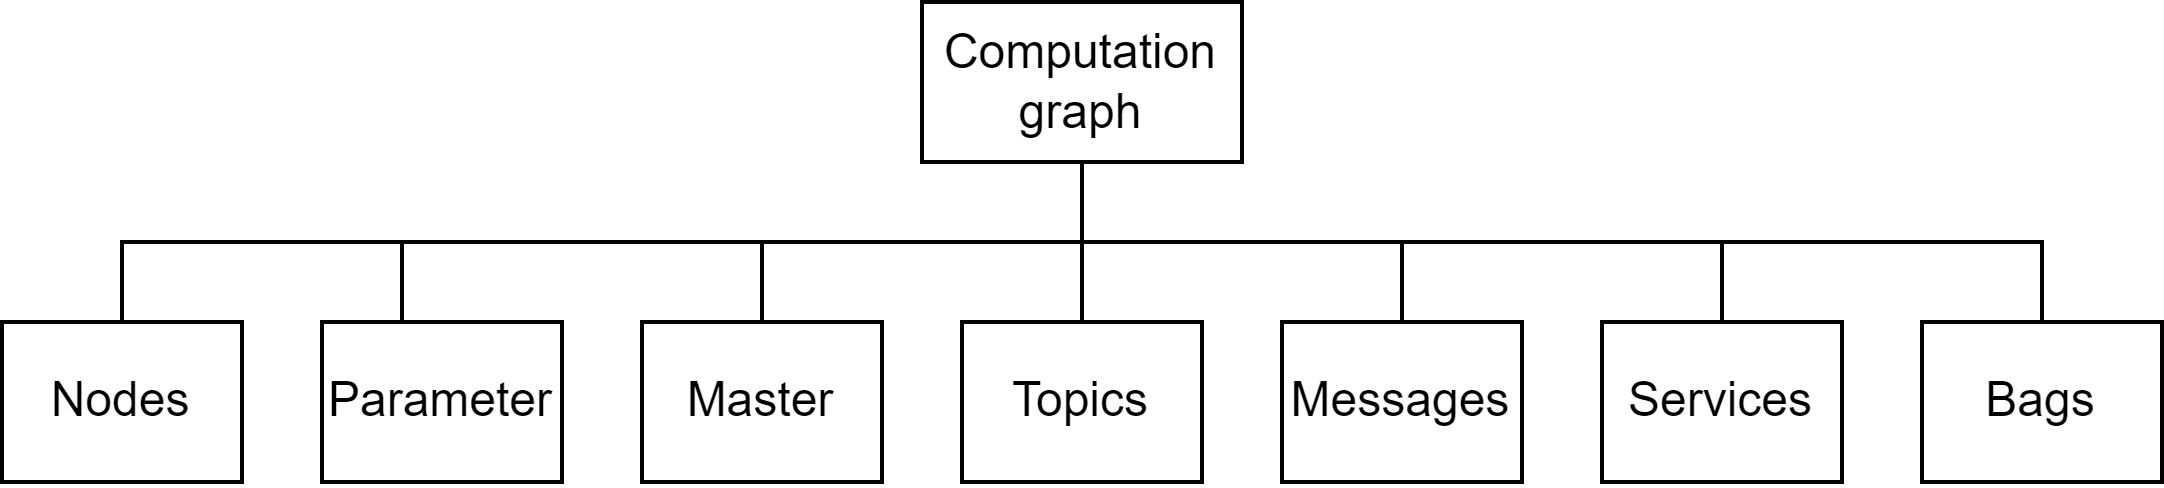
\includegraphics[width=0.75\linewidth]{images/cg.png}
    \caption{ROS computational graph}
\end{figure}

\subsection{Nodes}
ROS executable units include Python scripts and C++ compiled source code. 
They are processes responsible for computation within the ROS framework. 
These units, referred to as nodes, exchange information through a graph structure. 
Nodes are designed to operate at a fine-grained scale and are integral components of robot systems, which are composed of multiple interconnected nodes.

\subsection{Master}
The ROS Master serves as the central hub, facilitating naming and registration services crucial for node interactions. 
In every system, including distributed architectures, there exists a single master.
This centralized entity enables ROS nodes to effectively locate each other.
\begin{figure}[H]
    \centering
    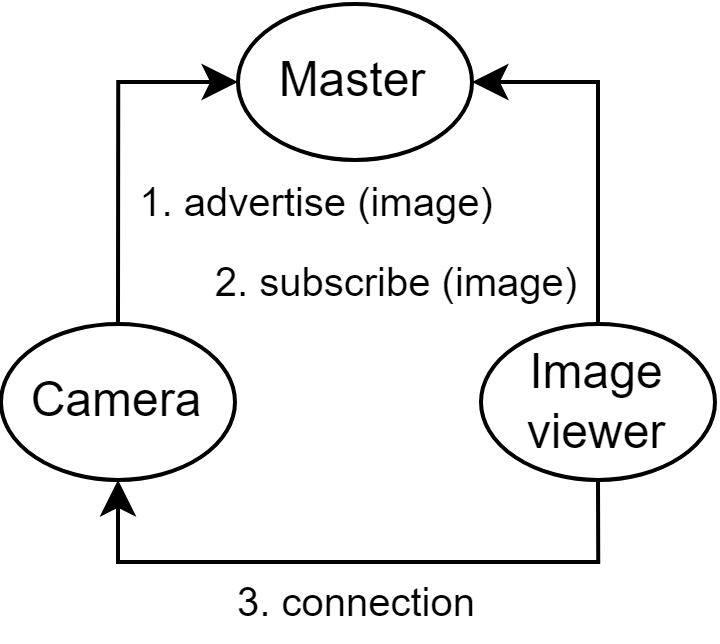
\includegraphics[width=0.5\linewidth]{images/master.png}
    \caption{ROS master}
\end{figure}
In this scenario, the camera node advertises the master with an image, making it available on a specific topic. 
Subsequently, the image viewer node subscribes to the same topic through the master.
Once the requested topic is found, the ROS master facilitates communication by providing the node name, allowing the subscriber to establish communication with the node that generated the image. 
This interaction demonstrates the pivotal role of the ROS master in mediating communication between nodes in the ROS ecosystem.

\subsection{Topics}
Topics serve as named channels for communication within the ROS framework, implementing the publish/subscribe paradigm. 
They facilitate communication between nodes by allowing multiple nodes to publish messages on a topic and multiple nodes to read those messages from the same topic. 
Topics are associated with specific message types, but they do not guarantee message delivery.

It's advisable to avoid scenarios where multiple talkers are connected to the same topic in ROS.\@
This is because ROS lacks a mechanism to discern the origin of a message in such cases.

\subsection{Messages}
Communication on topics involves the exchange of messages, which define the type of information being transmitted. 
A wide range of predefined message types is available.
Additionally, it is possible to create custom messages using a straightforward language. 
These custom messages can incorporate existing message types along with base types as needed.

\subsection{Services}
Services function akin to remote function calls within ROS, adhering to the client/server paradigm. 
When a service call is made, the code waits for its completion, ensuring a guarantee of execution. 
Services utilize message structures for their operation.

\subsection{Parameter server}
The parameter server is a shared, network-accessible multivariable dictionary utilized by nodes for storing and accessing parameters during runtime. 
It's not optimized for performance or data exchange. 
This server is linked to the master, constituting one of the functionalities provided by ROScore.
The parameter server can store a range of data types, including 32-bit integer, Boolean, string, double, ISO8601 date, and base64-encoded binary data.

\subsection{Bags}
Bags serve as a file format (*.bag) designed for storing and replaying messages within ROS.\@ 
They constitute the primary mechanism for data logging, capable of recording all exchanges occurring on the ROS graph, including messages, services, parameters, and actions. 
Bags are essential tools for data analysis, storage, visualization, and algorithm testing within the ROS ecosystem.

\subsection{ROScore}
ROScore is a foundational component of ROS-based systems, comprising nodes and programs essential for operation. 
It must be active to facilitate communication among ROS nodes. 
Launching ROScore via the command initiates its elements, which include a ROS master, a ROS parameter server, and a ROSout logging node.